% Created by tikzDevice version 0.6.1 on 2016-02-24 14:10:25
% !TEX encoding = UTF-8 Unicode
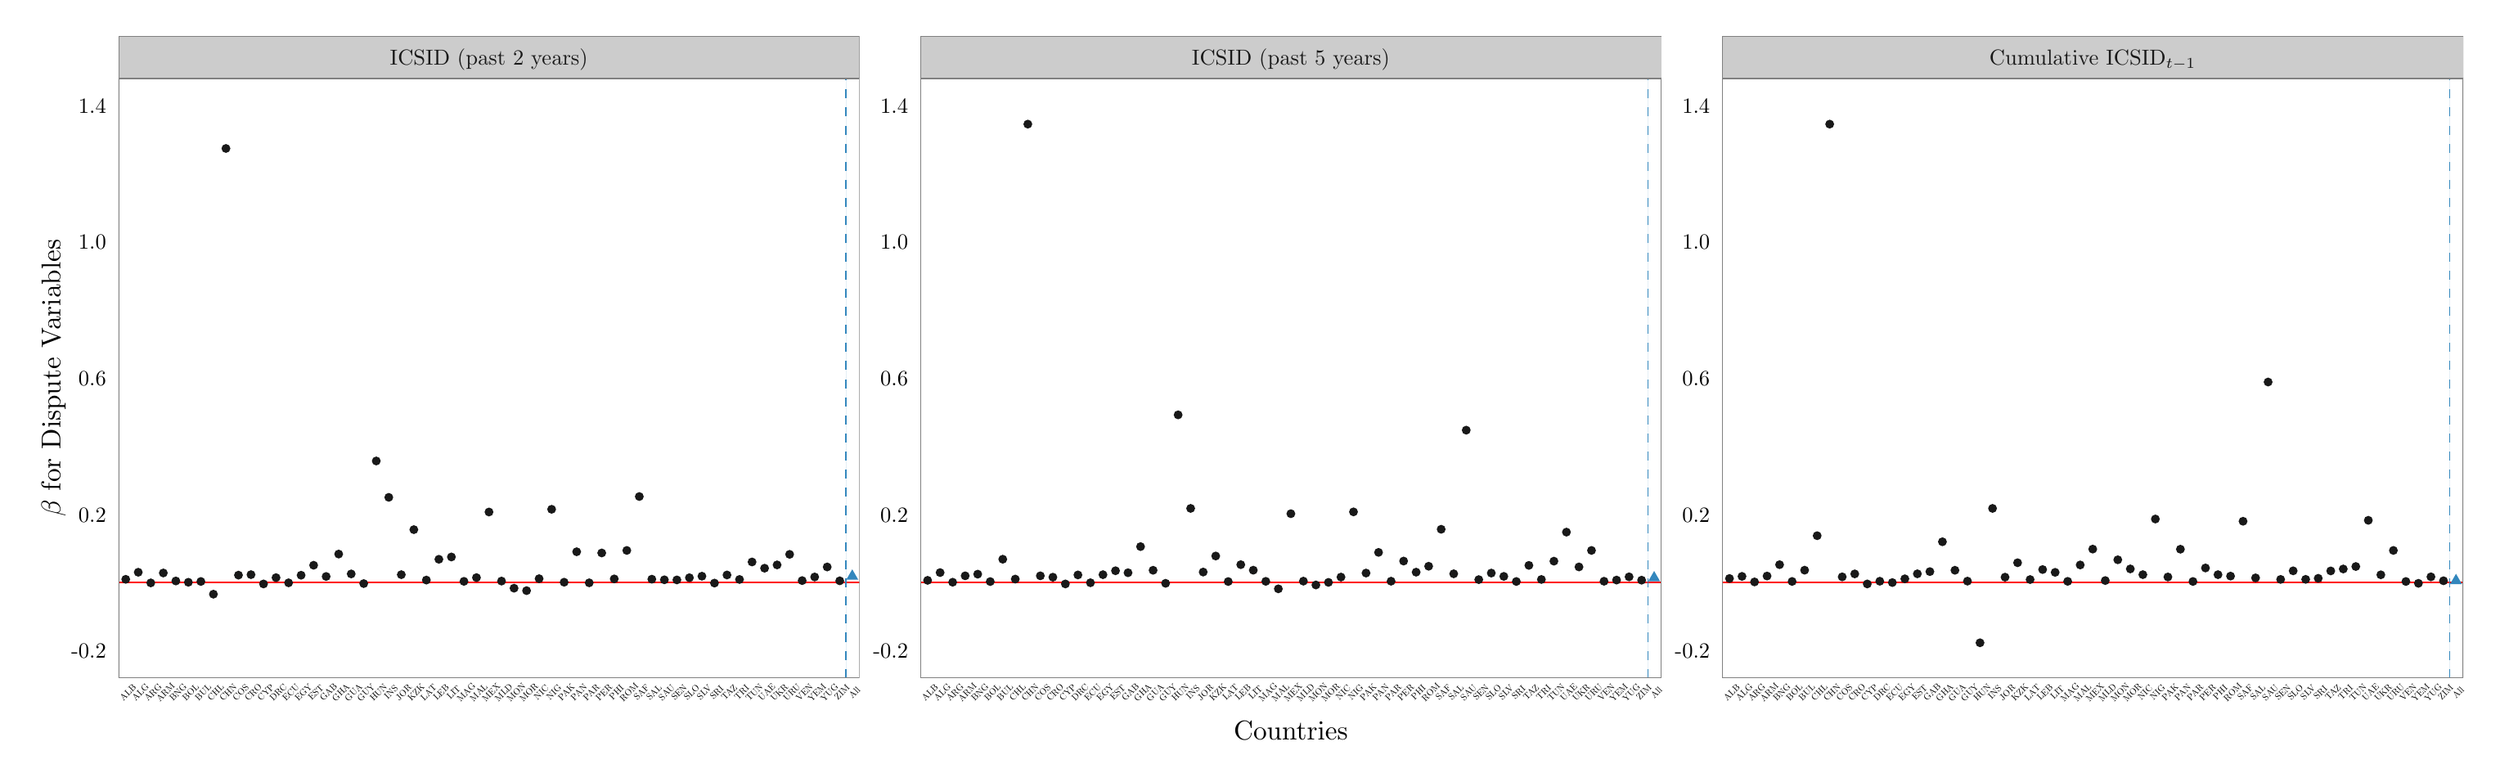
\begin{tikzpicture}[x=1pt,y=1pt]
\definecolor[named]{drawColor}{rgb}{0.00,0.00,0.00}
\definecolor[named]{fillColor}{rgb}{1.00,1.00,1.00}
\fill[color=fillColor,] (0,0) rectangle (1084.05,325.21);
\begin{scope}
\path[clip] (  0.00,  0.00) rectangle (1084.05,325.21);
\end{scope}
\begin{scope}
\path[clip] (  0.00,  0.00) rectangle (1084.05,325.21);
\end{scope}
\begin{scope}
\path[clip] (  0.00,  0.00) rectangle (1084.05,325.21);
\end{scope}
\begin{scope}
\path[clip] (  0.00,  0.00) rectangle (1084.05,325.21);
\end{scope}
\begin{scope}
\path[clip] (  0.00,  0.00) rectangle (1084.05,325.21);
\end{scope}
\begin{scope}
\path[clip] (  0.00,  0.00) rectangle (1084.05,325.21);
\end{scope}
\begin{scope}
\path[clip] (  0.00,  0.00) rectangle (1084.05,325.21);
\end{scope}
\begin{scope}
\path[clip] (  0.00,  0.00) rectangle (1084.05,325.21);
\end{scope}
\begin{scope}
\path[clip] (  0.00,  0.00) rectangle (1084.05,325.21);
\end{scope}
\begin{scope}
\path[clip] (  0.00,  0.00) rectangle (1084.05,325.21);
\end{scope}
\begin{scope}
\path[clip] (  0.00,  0.00) rectangle (1084.05,325.21);
\end{scope}
\begin{scope}
\path[clip] (  0.00,  0.00) rectangle (1084.05,325.21);
\end{scope}
\begin{scope}
\path[clip] (  0.00,  0.00) rectangle (1084.05,325.21);
\end{scope}
\begin{scope}
\path[clip] (  0.00,  0.00) rectangle (1084.05,325.21);
\end{scope}
\begin{scope}
\path[clip] (  0.00,  0.00) rectangle (1084.05,325.21);
\end{scope}
\begin{scope}
\path[clip] (  0.00,  0.00) rectangle (1084.05,325.21);
\definecolor[named]{drawColor}{rgb}{1.00,1.00,1.00}
\definecolor[named]{fillColor}{rgb}{1.00,1.00,1.00}

\draw[color=drawColor,line width= 0.6pt,line cap=round,line join=round,fill=fillColor,] (  0.00,  0.00) rectangle (1084.05,325.21);
\end{scope}
\begin{scope}
\path[clip] (  0.00,  0.00) rectangle (1084.05,325.21);
\end{scope}
\begin{scope}
\path[clip] ( 42.33, 35.72) rectangle (369.66,300.60);
\definecolor[named]{fillColor}{rgb}{1.00,1.00,1.00}

\draw[fill=fillColor,draw opacity=0.00,] ( 42.33, 35.72) rectangle (369.66,300.60);
\definecolor[named]{drawColor}{rgb}{1.00,0.00,0.00}
\definecolor[named]{fillColor}{rgb}{1.00,0.00,0.00}

\draw[color=drawColor,line width= 0.6pt,line join=round,fill=fillColor,] ( 42.33, 77.86) -- (369.66, 77.86);
\definecolor[named]{fillColor}{rgb}{0.10,0.10,0.10}

\draw[fill=fillColor,draw opacity=0.00,] (316.65, 79.23) circle (  1.96);

\draw[fill=fillColor,draw opacity=0.00,] (205.99,109.03) circle (  1.96);

\draw[fill=fillColor,draw opacity=0.00,] (145.13, 81.68) circle (  1.96);

\draw[fill=fillColor,draw opacity=0.00,] (277.92, 79.35) circle (  1.96);

\draw[fill=fillColor,draw opacity=0.00,] (228.13, 79.57) circle (  1.96);

\draw[fill=fillColor,draw opacity=0.00,] ( 95.33, 81.14) circle (  1.96);

\draw[fill=fillColor,draw opacity=0.00,] (244.72, 91.47) circle (  1.96);

\draw[fill=fillColor,draw opacity=0.00,] (344.32, 78.73) circle (  1.96);

\draw[fill=fillColor,draw opacity=0.00,] (150.66, 77.41) circle (  1.96);

\draw[fill=fillColor,draw opacity=0.00,] (117.47, 77.75) circle (  1.96);

\draw[fill=fillColor,draw opacity=0.00,] (255.79, 90.94) circle (  1.96);

\draw[fill=fillColor,draw opacity=0.00,] ( 73.20, 77.99) circle (  1.96);

\draw[fill=fillColor,draw opacity=0.00,] (250.26, 77.75) circle (  1.96);

\draw[fill=fillColor,draw opacity=0.00,] ( 84.27, 72.73) circle (  1.96);

\draw[fill=fillColor,draw opacity=0.00,] ( 56.60, 77.72) circle (  1.96);

\draw[fill=fillColor,draw opacity=0.00,] (338.79, 90.32) circle (  1.96);

\draw[fill=fillColor,draw opacity=0.00,] (156.20,131.57) circle (  1.96);

\draw[fill=fillColor,draw opacity=0.00,] (294.52, 80.00) circle (  1.96);

\draw[fill=fillColor,draw opacity=0.00,] ( 45.54, 79.30) circle (  1.96);

\draw[fill=fillColor,draw opacity=0.00,] (100.87, 81.36) circle (  1.96);

\draw[fill=fillColor,draw opacity=0.00,] (355.38, 84.75) circle (  1.96);

\draw[fill=fillColor,draw opacity=0.00,] (300.05, 80.67) circle (  1.96);

\draw[fill=fillColor,draw opacity=0.00,] (106.40, 77.25) circle (  1.96);

\draw[fill=fillColor,draw opacity=0.00,] ( 78.73, 78.34) circle (  1.96);

\draw[fill=fillColor,draw opacity=0.00,] (211.53, 78.52) circle (  1.96);

\draw[fill=fillColor,draw opacity=0.00,] (266.86, 92.05) circle (  1.96);

\draw[fill=fillColor,draw opacity=0.00,] (128.53, 85.51) circle (  1.96);

\draw[fill=fillColor,draw opacity=0.00,] (178.33, 78.96) circle (  1.96);

\draw[fill=fillColor,draw opacity=0.00,] (189.39, 89.17) circle (  1.96);

\draw[fill=fillColor,draw opacity=0.00,] (333.25, 85.66) circle (  1.96);

\draw[fill=fillColor,draw opacity=0.00,] ( 62.14, 82.10) circle (  1.96);

\draw[fill=fillColor,draw opacity=0.00,] (288.99, 79.03) circle (  1.96);

\draw[fill=fillColor,draw opacity=0.00,] (139.60, 90.45) circle (  1.96);

\draw[fill=fillColor,draw opacity=0.00,] (233.66,110.23) circle (  1.96);

\draw[fill=fillColor,draw opacity=0.00,] (134.06, 80.55) circle (  1.96);

\draw[fill=fillColor,draw opacity=0.00,] (111.93, 80.03) circle (  1.96);

\draw[fill=fillColor,draw opacity=0.00,] (311.12, 81.21) circle (  1.96);

\draw[fill=fillColor,draw opacity=0.00,] (360.92, 78.63) circle (  1.96);

\draw[fill=fillColor,draw opacity=0.00,] (272.39,115.86) circle (  1.96);

\draw[fill=fillColor,draw opacity=0.00,] (194.93, 78.40) circle (  1.96);

\draw[fill=fillColor,draw opacity=0.00,] (222.59, 74.29) circle (  1.96);

\draw[fill=fillColor,draw opacity=0.00,] ( 51.07, 82.41) circle (  1.96);

\draw[fill=fillColor,draw opacity=0.00,] (322.19, 86.96) circle (  1.96);

\draw[fill=fillColor,draw opacity=0.00,] (123.00, 81.10) circle (  1.96);

\draw[fill=fillColor,draw opacity=0.00,] (183.86, 88.14) circle (  1.96);

\draw[fill=fillColor,draw opacity=0.00,] (167.26, 81.35) circle (  1.96);

\draw[fill=fillColor,draw opacity=0.00,] (283.46, 79.08) circle (  1.96);

\draw[fill=fillColor,draw opacity=0.00,] (349.85, 80.33) circle (  1.96);

\draw[fill=fillColor,draw opacity=0.00,] (327.72, 84.20) circle (  1.96);

\draw[fill=fillColor,draw opacity=0.00,] (172.80,101.24) circle (  1.96);

\draw[fill=fillColor,draw opacity=0.00,] ( 89.80,269.62) circle (  1.96);

\draw[fill=fillColor,draw opacity=0.00,] (217.06, 75.37) circle (  1.96);

\draw[fill=fillColor,draw opacity=0.00,] (239.19, 78.01) circle (  1.96);

\draw[fill=fillColor,draw opacity=0.00,] ( 67.67, 78.56) circle (  1.96);

\draw[fill=fillColor,draw opacity=0.00,] (305.59, 77.63) circle (  1.96);

\draw[fill=fillColor,draw opacity=0.00,] (200.46, 80.05) circle (  1.96);

\draw[fill=fillColor,draw opacity=0.00,] (261.32, 79.48) circle (  1.96);

\draw[fill=fillColor,draw opacity=0.00,] (161.73,115.50) circle (  1.96);
\definecolor[named]{fillColor}{rgb}{0.20,0.53,0.74}

\draw[fill=fillColor,draw opacity=0.00,] (366.45, 83.71) --
	(369.09, 79.13) --
	(363.81, 79.13) --
	cycle;
\definecolor[named]{drawColor}{rgb}{0.20,0.53,0.74}

\draw[color=drawColor,line width= 0.6pt,dash pattern=on 4pt off 4pt ,line join=round,fill=fillColor,] (363.68, 35.72) -- (363.68,300.60);
\definecolor[named]{drawColor}{rgb}{0.50,0.50,0.50}

\draw[color=drawColor,line width= 0.6pt,line cap=round,line join=round,fill opacity=0.00,] ( 42.33, 35.72) rectangle (369.66,300.60);
\end{scope}
\begin{scope}
\path[clip] (  0.00,  0.00) rectangle (1084.05,325.21);
\end{scope}
\begin{scope}
\path[clip] (396.52, 35.72) rectangle (723.85,300.60);
\definecolor[named]{fillColor}{rgb}{1.00,1.00,1.00}

\draw[fill=fillColor,draw opacity=0.00,] (396.52, 35.72) rectangle (723.85,300.60);
\definecolor[named]{drawColor}{rgb}{1.00,0.00,0.00}
\definecolor[named]{fillColor}{rgb}{1.00,0.00,0.00}

\draw[color=drawColor,line width= 0.6pt,line join=round,fill=fillColor,] (396.52, 77.86) -- (723.85, 77.86);
\definecolor[named]{fillColor}{rgb}{0.10,0.10,0.10}

\draw[fill=fillColor,draw opacity=0.00,] (670.85, 79.23) circle (  1.96);

\draw[fill=fillColor,draw opacity=0.00,] (560.19,108.28) circle (  1.96);

\draw[fill=fillColor,draw opacity=0.00,] (499.33, 83.29) circle (  1.96);

\draw[fill=fillColor,draw opacity=0.00,] (632.12, 81.74) circle (  1.96);

\draw[fill=fillColor,draw opacity=0.00,] (582.32, 80.28) circle (  1.96);

\draw[fill=fillColor,draw opacity=0.00,] (449.53, 80.84) circle (  1.96);

\draw[fill=fillColor,draw opacity=0.00,] (598.92, 91.19) circle (  1.96);

\draw[fill=fillColor,draw opacity=0.00,] (698.51, 78.44) circle (  1.96);

\draw[fill=fillColor,draw opacity=0.00,] (504.86, 77.53) circle (  1.96);

\draw[fill=fillColor,draw opacity=0.00,] (471.66, 77.78) circle (  1.96);

\draw[fill=fillColor,draw opacity=0.00,] (609.99, 87.36) circle (  1.96);

\draw[fill=fillColor,draw opacity=0.00,] (427.40, 78.30) circle (  1.96);

\draw[fill=fillColor,draw opacity=0.00,] (604.45, 78.46) circle (  1.96);

\draw[fill=fillColor,draw opacity=0.00,] (438.46, 79.40) circle (  1.96);

\draw[fill=fillColor,draw opacity=0.00,] (410.80, 78.01) circle (  1.96);

\draw[fill=fillColor,draw opacity=0.00,] (692.98, 92.05) circle (  1.96);

\draw[fill=fillColor,draw opacity=0.00,] (510.39,151.94) circle (  1.96);

\draw[fill=fillColor,draw opacity=0.00,] (648.72, 82.05) circle (  1.96);

\draw[fill=fillColor,draw opacity=0.00,] (399.73, 78.84) circle (  1.96);

\draw[fill=fillColor,draw opacity=0.00,] (455.06, 80.23) circle (  1.96);

\draw[fill=fillColor,draw opacity=0.00,] (709.58, 80.39) circle (  1.96);

\draw[fill=fillColor,draw opacity=0.00,] (654.25, 80.59) circle (  1.96);

\draw[fill=fillColor,draw opacity=0.00,] (460.59, 77.25) circle (  1.96);

\draw[fill=fillColor,draw opacity=0.00,] (432.93, 88.17) circle (  1.96);

\draw[fill=fillColor,draw opacity=0.00,] (565.72, 78.49) circle (  1.96);

\draw[fill=fillColor,draw opacity=0.00,] (621.05, 85.07) circle (  1.96);

\draw[fill=fillColor,draw opacity=0.00,] (482.73, 83.08) circle (  1.96);

\draw[fill=fillColor,draw opacity=0.00,] (532.52, 78.31) circle (  1.96);

\draw[fill=fillColor,draw opacity=0.00,] (543.59, 83.32) circle (  1.96);

\draw[fill=fillColor,draw opacity=0.00,] (687.45, 84.76) circle (  1.96);

\draw[fill=fillColor,draw opacity=0.00,] (416.33, 80.84) circle (  1.96);

\draw[fill=fillColor,draw opacity=0.00,] (643.18, 79.16) circle (  1.96);

\draw[fill=fillColor,draw opacity=0.00,] (493.79, 93.74) circle (  1.96);

\draw[fill=fillColor,draw opacity=0.00,] (587.85,109.09) circle (  1.96);

\draw[fill=fillColor,draw opacity=0.00,] (488.26, 82.20) circle (  1.96);

\draw[fill=fillColor,draw opacity=0.00,] (466.13, 81.23) circle (  1.96);

\draw[fill=fillColor,draw opacity=0.00,] (665.32, 85.45) circle (  1.96);

\draw[fill=fillColor,draw opacity=0.00,] (715.11, 78.91) circle (  1.96);

\draw[fill=fillColor,draw opacity=0.00,] (626.58,101.40) circle (  1.96);

\draw[fill=fillColor,draw opacity=0.00,] (549.12, 78.40) circle (  1.96);

\draw[fill=fillColor,draw opacity=0.00,] (576.79, 77.95) circle (  1.96);

\draw[fill=fillColor,draw opacity=0.00,] (405.26, 82.27) circle (  1.96);

\draw[fill=fillColor,draw opacity=0.00,] (676.38, 87.31) circle (  1.96);

\draw[fill=fillColor,draw opacity=0.00,] (477.19, 81.34) circle (  1.96);

\draw[fill=fillColor,draw opacity=0.00,] (538.06, 85.77) circle (  1.96);

\draw[fill=fillColor,draw opacity=0.00,] (521.46, 82.50) circle (  1.96);

\draw[fill=fillColor,draw opacity=0.00,] (637.65,145.18) circle (  1.96);

\draw[fill=fillColor,draw opacity=0.00,] (704.05, 78.96) circle (  1.96);

\draw[fill=fillColor,draw opacity=0.00,] (681.91,100.14) circle (  1.96);

\draw[fill=fillColor,draw opacity=0.00,] (526.99, 89.59) circle (  1.96);

\draw[fill=fillColor,draw opacity=0.00,] (444.00,280.37) circle (  1.96);

\draw[fill=fillColor,draw opacity=0.00,] (571.25, 76.80) circle (  1.96);

\draw[fill=fillColor,draw opacity=0.00,] (593.39, 82.06) circle (  1.96);

\draw[fill=fillColor,draw opacity=0.00,] (421.86, 81.57) circle (  1.96);

\draw[fill=fillColor,draw opacity=0.00,] (659.78, 78.33) circle (  1.96);

\draw[fill=fillColor,draw opacity=0.00,] (554.66, 75.09) circle (  1.96);

\draw[fill=fillColor,draw opacity=0.00,] (615.52, 82.45) circle (  1.96);

\draw[fill=fillColor,draw opacity=0.00,] (515.92,110.62) circle (  1.96);
\definecolor[named]{fillColor}{rgb}{0.20,0.53,0.74}

\draw[fill=fillColor,draw opacity=0.00,] (720.65, 82.97) --
	(723.29, 78.39) --
	(718.00, 78.39) --
	cycle;
\definecolor[named]{drawColor}{rgb}{0.20,0.53,0.74}

\draw[color=drawColor,line width= 0.6pt,dash pattern=on 4pt off 4pt ,line join=round,fill=fillColor,] (717.88, 35.72) -- (717.88,300.60);
\definecolor[named]{drawColor}{rgb}{0.50,0.50,0.50}

\draw[color=drawColor,line width= 0.6pt,line cap=round,line join=round,fill opacity=0.00,] (396.52, 35.72) rectangle (723.85,300.60);
\end{scope}
\begin{scope}
\path[clip] (  0.00,  0.00) rectangle (1084.05,325.21);
\end{scope}
\begin{scope}
\path[clip] (750.72, 35.72) rectangle (1078.05,300.60);
\definecolor[named]{fillColor}{rgb}{1.00,1.00,1.00}

\draw[fill=fillColor,draw opacity=0.00,] (750.72, 35.72) rectangle (1078.05,300.60);
\definecolor[named]{drawColor}{rgb}{1.00,0.00,0.00}
\definecolor[named]{fillColor}{rgb}{1.00,0.00,0.00}

\draw[color=drawColor,line width= 0.6pt,line join=round,fill=fillColor,] (750.72, 77.86) -- (1078.05, 77.86);
\definecolor[named]{fillColor}{rgb}{0.10,0.10,0.10}

\draw[fill=fillColor,draw opacity=0.00,] (1025.04, 83.86) circle (  1.96);

\draw[fill=fillColor,draw opacity=0.00,] (914.38, 92.64) circle (  1.96);

\draw[fill=fillColor,draw opacity=0.00,] (853.52, 83.29) circle (  1.96);

\draw[fill=fillColor,draw opacity=0.00,] (986.31, 79.93) circle (  1.96);

\draw[fill=fillColor,draw opacity=0.00,] (936.52, 81.36) circle (  1.96);

\draw[fill=fillColor,draw opacity=0.00,] (803.72, 80.38) circle (  1.96);

\draw[fill=fillColor,draw opacity=0.00,] (953.11, 92.59) circle (  1.96);

\draw[fill=fillColor,draw opacity=0.00,] (1052.71, 78.34) circle (  1.96);

\draw[fill=fillColor,draw opacity=0.00,] (859.05, 78.49) circle (  1.96);

\draw[fill=fillColor,draw opacity=0.00,] (825.86, 77.86) circle (  1.96);

\draw[fill=fillColor,draw opacity=0.00,] (964.18, 84.31) circle (  1.96);

\draw[fill=fillColor,draw opacity=0.00,] (781.59, 78.35) circle (  1.96);

\draw[fill=fillColor,draw opacity=0.00,] (958.65, 78.34) circle (  1.96);

\draw[fill=fillColor,draw opacity=0.00,] (792.66, 98.56) circle (  1.96);

\draw[fill=fillColor,draw opacity=0.00,] (764.99, 78.14) circle (  1.96);

\draw[fill=fillColor,draw opacity=0.00,] (1047.18, 92.05) circle (  1.96);

\draw[fill=fillColor,draw opacity=0.00,] (864.59, 51.26) circle (  1.96);

\draw[fill=fillColor,draw opacity=0.00,] (1002.91, 83.04) circle (  1.96);

\draw[fill=fillColor,draw opacity=0.00,] (753.93, 79.66) circle (  1.96);

\draw[fill=fillColor,draw opacity=0.00,] (809.26, 81.69) circle (  1.96);

\draw[fill=fillColor,draw opacity=0.00,] (1063.77, 80.39) circle (  1.96);

\draw[fill=fillColor,draw opacity=0.00,] (1008.44, 79.28) circle (  1.96);

\draw[fill=fillColor,draw opacity=0.00,] (814.79, 77.25) circle (  1.96);

\draw[fill=fillColor,draw opacity=0.00,] (787.12, 83.33) circle (  1.96);

\draw[fill=fillColor,draw opacity=0.00,] (919.92, 78.75) circle (  1.96);

\draw[fill=fillColor,draw opacity=0.00,] (975.25, 80.71) circle (  1.96);

\draw[fill=fillColor,draw opacity=0.00,] (836.92, 81.73) circle (  1.96);

\draw[fill=fillColor,draw opacity=0.00,] (886.72, 79.19) circle (  1.96);

\draw[fill=fillColor,draw opacity=0.00,] (897.78, 82.37) circle (  1.96);

\draw[fill=fillColor,draw opacity=0.00,] (1041.64, 81.29) circle (  1.96);

\draw[fill=fillColor,draw opacity=0.00,] (770.53, 80.75) circle (  1.96);

\draw[fill=fillColor,draw opacity=0.00,] (997.38, 79.25) circle (  1.96);

\draw[fill=fillColor,draw opacity=0.00,] (847.99, 95.88) circle (  1.96);

\draw[fill=fillColor,draw opacity=0.00,] (942.05,105.93) circle (  1.96);

\draw[fill=fillColor,draw opacity=0.00,] (842.45, 82.70) circle (  1.96);

\draw[fill=fillColor,draw opacity=0.00,] (820.32, 78.45) circle (  1.96);

\draw[fill=fillColor,draw opacity=0.00,] (1019.51, 83.01) circle (  1.96);

\draw[fill=fillColor,draw opacity=0.00,] (1069.31, 78.65) circle (  1.96);

\draw[fill=fillColor,draw opacity=0.00,] (980.78,104.94) circle (  1.96);

\draw[fill=fillColor,draw opacity=0.00,] (903.32, 78.40) circle (  1.96);

\draw[fill=fillColor,draw opacity=0.00,] (930.98, 83.89) circle (  1.96);

\draw[fill=fillColor,draw opacity=0.00,] (759.46, 80.59) circle (  1.96);

\draw[fill=fillColor,draw opacity=0.00,] (1030.58, 84.95) circle (  1.96);

\draw[fill=fillColor,draw opacity=0.00,] (831.39, 79.52) circle (  1.96);

\draw[fill=fillColor,draw opacity=0.00,] (892.25, 83.61) circle (  1.96);

\draw[fill=fillColor,draw opacity=0.00,] (875.65, 80.24) circle (  1.96);

\draw[fill=fillColor,draw opacity=0.00,] (991.85,166.45) circle (  1.96);

\draw[fill=fillColor,draw opacity=0.00,] (1058.24, 77.53) circle (  1.96);

\draw[fill=fillColor,draw opacity=0.00,] (1036.11,105.36) circle (  1.96);

\draw[fill=fillColor,draw opacity=0.00,] (881.19, 86.62) circle (  1.96);

\draw[fill=fillColor,draw opacity=0.00,] (798.19,280.37) circle (  1.96);

\draw[fill=fillColor,draw opacity=0.00,] (925.45, 87.92) circle (  1.96);

\draw[fill=fillColor,draw opacity=0.00,] (947.58, 80.33) circle (  1.96);

\draw[fill=fillColor,draw opacity=0.00,] (776.06, 85.76) circle (  1.96);

\draw[fill=fillColor,draw opacity=0.00,] (1013.98, 79.74) circle (  1.96);

\draw[fill=fillColor,draw opacity=0.00,] (908.85, 85.64) circle (  1.96);

\draw[fill=fillColor,draw opacity=0.00,] (969.71, 81.35) circle (  1.96);

\draw[fill=fillColor,draw opacity=0.00,] (870.12,110.62) circle (  1.96);
\definecolor[named]{fillColor}{rgb}{0.20,0.53,0.74}

\draw[fill=fillColor,draw opacity=0.00,] (1074.84, 81.73) --
	(1077.48, 77.15) --
	(1072.20, 77.15) --
	cycle;
\definecolor[named]{drawColor}{rgb}{0.20,0.53,0.74}

\draw[color=drawColor,line width= 0.6pt,dash pattern=on 4pt off 4pt ,line join=round,fill=fillColor,] (1072.07, 35.72) -- (1072.07,300.60);
\definecolor[named]{drawColor}{rgb}{0.50,0.50,0.50}

\draw[color=drawColor,line width= 0.6pt,line cap=round,line join=round,fill opacity=0.00,] (750.72, 35.72) rectangle (1078.05,300.60);
\end{scope}
\begin{scope}
\path[clip] (  0.00,  0.00) rectangle (1084.05,325.21);
\end{scope}
\begin{scope}
\path[clip] (  0.00,  0.00) rectangle (1084.05,325.21);
\end{scope}
\begin{scope}
\path[clip] (  0.00,  0.00) rectangle (1084.05,325.21);
\end{scope}
\begin{scope}
\path[clip] ( 42.33,300.60) rectangle (369.66,319.21);
\definecolor[named]{drawColor}{rgb}{0.50,0.50,0.50}
\definecolor[named]{fillColor}{rgb}{0.80,0.80,0.80}

\draw[color=drawColor,line width= 0.2pt,line cap=round,line join=round,fill=fillColor,] ( 42.33,300.60) rectangle (369.66,319.21);
\definecolor[named]{drawColor}{rgb}{0.10,0.10,0.10}

\node[color=drawColor,anchor=base,inner sep=0pt, outer sep=0pt, scale=  0.96] at (205.99,306.60) {ICSID  (past 2 years)%
};
\end{scope}
\begin{scope}
\path[clip] ( 42.33,300.60) rectangle (369.66,319.21);
\end{scope}
\begin{scope}
\path[clip] (  0.00,  0.00) rectangle (1084.05,325.21);
\end{scope}
\begin{scope}
\path[clip] (  0.00,  0.00) rectangle (1084.05,325.21);
\end{scope}
\begin{scope}
\path[clip] (  0.00,  0.00) rectangle (1084.05,325.21);
\end{scope}
\begin{scope}
\path[clip] (  0.00,  0.00) rectangle (1084.05,325.21);
\end{scope}
\begin{scope}
\path[clip] (  0.00,  0.00) rectangle (1084.05,325.21);
\end{scope}
\begin{scope}
\path[clip] (  0.00,  0.00) rectangle (1084.05,325.21);
\end{scope}
\begin{scope}
\path[clip] (396.52,300.60) rectangle (723.85,319.21);
\definecolor[named]{drawColor}{rgb}{0.50,0.50,0.50}
\definecolor[named]{fillColor}{rgb}{0.80,0.80,0.80}

\draw[color=drawColor,line width= 0.2pt,line cap=round,line join=round,fill=fillColor,] (396.52,300.60) rectangle (723.85,319.21);
\definecolor[named]{drawColor}{rgb}{0.10,0.10,0.10}

\node[color=drawColor,anchor=base,inner sep=0pt, outer sep=0pt, scale=  0.96] at (560.19,306.60) {ICSID  (past 5 years)%
};
\end{scope}
\begin{scope}
\path[clip] (396.52,300.60) rectangle (723.85,319.21);
\end{scope}
\begin{scope}
\path[clip] (  0.00,  0.00) rectangle (1084.05,325.21);
\end{scope}
\begin{scope}
\path[clip] (  0.00,  0.00) rectangle (1084.05,325.21);
\end{scope}
\begin{scope}
\path[clip] (  0.00,  0.00) rectangle (1084.05,325.21);
\end{scope}
\begin{scope}
\path[clip] (  0.00,  0.00) rectangle (1084.05,325.21);
\end{scope}
\begin{scope}
\path[clip] (  0.00,  0.00) rectangle (1084.05,325.21);
\end{scope}
\begin{scope}
\path[clip] (  0.00,  0.00) rectangle (1084.05,325.21);
\end{scope}
\begin{scope}
\path[clip] (750.72,300.60) rectangle (1078.05,319.21);
\definecolor[named]{drawColor}{rgb}{0.50,0.50,0.50}
\definecolor[named]{fillColor}{rgb}{0.80,0.80,0.80}

\draw[color=drawColor,line width= 0.2pt,line cap=round,line join=round,fill=fillColor,] (750.72,300.60) rectangle (1078.05,319.21);
\definecolor[named]{drawColor}{rgb}{0.10,0.10,0.10}

\node[color=drawColor,anchor=base,inner sep=0pt, outer sep=0pt, scale=  0.96] at (914.38,306.60) {Cumulative ICSID$_{t-1}$%
};
\end{scope}
\begin{scope}
\path[clip] (750.72,300.60) rectangle (1078.05,319.21);
\end{scope}
\begin{scope}
\path[clip] (  0.00,  0.00) rectangle (1084.05,325.21);
\end{scope}
\begin{scope}
\path[clip] (  0.00,  0.00) rectangle (1084.05,325.21);
\end{scope}
\begin{scope}
\path[clip] (  0.00,  0.00) rectangle (1084.05,325.21);
\end{scope}
\begin{scope}
\path[clip] (  0.00,  0.00) rectangle (1084.05,325.21);
\end{scope}
\begin{scope}
\path[clip] (  0.00,  0.00) rectangle (1084.05,325.21);
\end{scope}
\begin{scope}
\path[clip] (  0.00,  0.00) rectangle (1084.05,325.21);
\end{scope}
\begin{scope}
\path[clip] (  0.00,  0.00) rectangle (1084.05,325.21);
\end{scope}
\begin{scope}
\path[clip] (  0.00,  0.00) rectangle (1084.05,325.21);
\end{scope}
\begin{scope}
\path[clip] (  0.00,  0.00) rectangle (1084.05,325.21);
\definecolor[named]{drawColor}{rgb}{0.00,0.00,0.00}

\node[color=drawColor,anchor=base east,inner sep=0pt, outer sep=0pt, scale=  0.96] at ( 36.93, 44.46) {-0.2%
};

\node[color=drawColor,anchor=base east,inner sep=0pt, outer sep=0pt, scale=  0.96] at ( 36.93,104.66) {0.2%
};

\node[color=drawColor,anchor=base east,inner sep=0pt, outer sep=0pt, scale=  0.96] at ( 36.93,164.86) {0.6%
};

\node[color=drawColor,anchor=base east,inner sep=0pt, outer sep=0pt, scale=  0.96] at ( 36.93,225.06) {1.0%
};

\node[color=drawColor,anchor=base east,inner sep=0pt, outer sep=0pt, scale=  0.96] at ( 36.93,285.26) {1.4%
};
\end{scope}
\begin{scope}
\path[clip] (  0.00,  0.00) rectangle (1084.05,325.21);
\end{scope}
\begin{scope}
\path[clip] (  0.00,  0.00) rectangle (1084.05,325.21);
\end{scope}
\begin{scope}
\path[clip] (  0.00,  0.00) rectangle (1084.05,325.21);
\end{scope}
\begin{scope}
\path[clip] (  0.00,  0.00) rectangle (1084.05,325.21);
\end{scope}
\begin{scope}
\path[clip] (  0.00,  0.00) rectangle (1084.05,325.21);
\end{scope}
\begin{scope}
\path[clip] (  0.00,  0.00) rectangle (1084.05,325.21);
\end{scope}
\begin{scope}
\path[clip] (  0.00,  0.00) rectangle (1084.05,325.21);
\end{scope}
\begin{scope}
\path[clip] (  0.00,  0.00) rectangle (1084.05,325.21);
\end{scope}
\begin{scope}
\path[clip] (  0.00,  0.00) rectangle (1084.05,325.21);
\end{scope}
\begin{scope}
\path[clip] (  0.00,  0.00) rectangle (1084.05,325.21);
\end{scope}
\begin{scope}
\path[clip] (  0.00,  0.00) rectangle (1084.05,325.21);
\end{scope}
\begin{scope}
\path[clip] (  0.00,  0.00) rectangle (1084.05,325.21);
\definecolor[named]{drawColor}{rgb}{0.00,0.00,0.00}

\node[color=drawColor,anchor=base east,inner sep=0pt, outer sep=0pt, scale=  0.96] at (391.12, 44.46) {-0.2%
};

\node[color=drawColor,anchor=base east,inner sep=0pt, outer sep=0pt, scale=  0.96] at (391.12,104.66) {0.2%
};

\node[color=drawColor,anchor=base east,inner sep=0pt, outer sep=0pt, scale=  0.96] at (391.12,164.86) {0.6%
};

\node[color=drawColor,anchor=base east,inner sep=0pt, outer sep=0pt, scale=  0.96] at (391.12,225.06) {1.0%
};

\node[color=drawColor,anchor=base east,inner sep=0pt, outer sep=0pt, scale=  0.96] at (391.12,285.26) {1.4%
};
\end{scope}
\begin{scope}
\path[clip] (  0.00,  0.00) rectangle (1084.05,325.21);
\end{scope}
\begin{scope}
\path[clip] (  0.00,  0.00) rectangle (1084.05,325.21);
\end{scope}
\begin{scope}
\path[clip] (  0.00,  0.00) rectangle (1084.05,325.21);
\end{scope}
\begin{scope}
\path[clip] (  0.00,  0.00) rectangle (1084.05,325.21);
\end{scope}
\begin{scope}
\path[clip] (  0.00,  0.00) rectangle (1084.05,325.21);
\end{scope}
\begin{scope}
\path[clip] (  0.00,  0.00) rectangle (1084.05,325.21);
\end{scope}
\begin{scope}
\path[clip] (  0.00,  0.00) rectangle (1084.05,325.21);
\end{scope}
\begin{scope}
\path[clip] (  0.00,  0.00) rectangle (1084.05,325.21);
\end{scope}
\begin{scope}
\path[clip] (  0.00,  0.00) rectangle (1084.05,325.21);
\end{scope}
\begin{scope}
\path[clip] (  0.00,  0.00) rectangle (1084.05,325.21);
\end{scope}
\begin{scope}
\path[clip] (  0.00,  0.00) rectangle (1084.05,325.21);
\end{scope}
\begin{scope}
\path[clip] (  0.00,  0.00) rectangle (1084.05,325.21);
\definecolor[named]{drawColor}{rgb}{0.00,0.00,0.00}

\node[color=drawColor,anchor=base east,inner sep=0pt, outer sep=0pt, scale=  0.96] at (745.32, 44.46) {-0.2%
};

\node[color=drawColor,anchor=base east,inner sep=0pt, outer sep=0pt, scale=  0.96] at (745.32,104.66) {0.2%
};

\node[color=drawColor,anchor=base east,inner sep=0pt, outer sep=0pt, scale=  0.96] at (745.32,164.86) {0.6%
};

\node[color=drawColor,anchor=base east,inner sep=0pt, outer sep=0pt, scale=  0.96] at (745.32,225.06) {1.0%
};

\node[color=drawColor,anchor=base east,inner sep=0pt, outer sep=0pt, scale=  0.96] at (745.32,285.26) {1.4%
};
\end{scope}
\begin{scope}
\path[clip] (  0.00,  0.00) rectangle (1084.05,325.21);
\end{scope}
\begin{scope}
\path[clip] (  0.00,  0.00) rectangle (1084.05,325.21);
\end{scope}
\begin{scope}
\path[clip] (  0.00,  0.00) rectangle (1084.05,325.21);
\end{scope}
\begin{scope}
\path[clip] (  0.00,  0.00) rectangle (1084.05,325.21);
\end{scope}
\begin{scope}
\path[clip] (  0.00,  0.00) rectangle (1084.05,325.21);
\end{scope}
\begin{scope}
\path[clip] (  0.00,  0.00) rectangle (1084.05,325.21);
\end{scope}
\begin{scope}
\path[clip] (  0.00,  0.00) rectangle (1084.05,325.21);
\end{scope}
\begin{scope}
\path[clip] (  0.00,  0.00) rectangle (1084.05,325.21);
\end{scope}
\begin{scope}
\path[clip] (  0.00,  0.00) rectangle (1084.05,325.21);
\end{scope}
\begin{scope}
\path[clip] (  0.00,  0.00) rectangle (1084.05,325.21);
\end{scope}
\begin{scope}
\path[clip] (  0.00,  0.00) rectangle (1084.05,325.21);
\end{scope}
\begin{scope}
\path[clip] (  0.00,  0.00) rectangle (1084.05,325.21);
\end{scope}
\begin{scope}
\path[clip] (  0.00,  0.00) rectangle (1084.05,325.21);
\end{scope}
\begin{scope}
\path[clip] (  0.00,  0.00) rectangle (1084.05,325.21);
\definecolor[named]{drawColor}{rgb}{0.00,0.00,0.00}

\node[rotate= 45.00,color=drawColor,anchor=base,inner sep=0pt, outer sep=0pt, scale=  0.40] at ( 47.48, 28.38) {ALB%
};

\node[rotate= 45.00,color=drawColor,anchor=base,inner sep=0pt, outer sep=0pt, scale=  0.40] at ( 53.02, 28.38) {ALG%
};

\node[rotate= 45.00,color=drawColor,anchor=base,inner sep=0pt, outer sep=0pt, scale=  0.40] at ( 58.55, 28.38) {ARG%
};

\node[rotate= 45.00,color=drawColor,anchor=base,inner sep=0pt, outer sep=0pt, scale=  0.40] at ( 64.08, 28.38) {ARM%
};

\node[rotate= 45.00,color=drawColor,anchor=base,inner sep=0pt, outer sep=0pt, scale=  0.40] at ( 69.62, 28.38) {BNG%
};

\node[rotate= 45.00,color=drawColor,anchor=base,inner sep=0pt, outer sep=0pt, scale=  0.40] at ( 75.15, 28.38) {BOL%
};

\node[rotate= 45.00,color=drawColor,anchor=base,inner sep=0pt, outer sep=0pt, scale=  0.40] at ( 80.68, 28.38) {BUL%
};

\node[rotate= 45.00,color=drawColor,anchor=base,inner sep=0pt, outer sep=0pt, scale=  0.40] at ( 86.22, 28.38) {CHL%
};

\node[rotate= 45.00,color=drawColor,anchor=base,inner sep=0pt, outer sep=0pt, scale=  0.40] at ( 91.75, 28.38) {CHN%
};

\node[rotate= 45.00,color=drawColor,anchor=base,inner sep=0pt, outer sep=0pt, scale=  0.40] at ( 97.28, 28.38) {COS%
};

\node[rotate= 45.00,color=drawColor,anchor=base,inner sep=0pt, outer sep=0pt, scale=  0.40] at (102.81, 28.38) {CRO%
};

\node[rotate= 45.00,color=drawColor,anchor=base,inner sep=0pt, outer sep=0pt, scale=  0.40] at (108.35, 28.38) {CYP%
};

\node[rotate= 45.00,color=drawColor,anchor=base,inner sep=0pt, outer sep=0pt, scale=  0.40] at (113.88, 28.38) {DRC%
};

\node[rotate= 45.00,color=drawColor,anchor=base,inner sep=0pt, outer sep=0pt, scale=  0.40] at (119.41, 28.38) {ECU%
};

\node[rotate= 45.00,color=drawColor,anchor=base,inner sep=0pt, outer sep=0pt, scale=  0.40] at (124.95, 28.38) {EGY%
};

\node[rotate= 45.00,color=drawColor,anchor=base,inner sep=0pt, outer sep=0pt, scale=  0.40] at (130.48, 28.38) {EST%
};

\node[rotate= 45.00,color=drawColor,anchor=base,inner sep=0pt, outer sep=0pt, scale=  0.40] at (136.01, 28.38) {GAB%
};

\node[rotate= 45.00,color=drawColor,anchor=base,inner sep=0pt, outer sep=0pt, scale=  0.40] at (141.55, 28.38) {GHA%
};

\node[rotate= 45.00,color=drawColor,anchor=base,inner sep=0pt, outer sep=0pt, scale=  0.40] at (147.08, 28.38) {GUA%
};

\node[rotate= 45.00,color=drawColor,anchor=base,inner sep=0pt, outer sep=0pt, scale=  0.40] at (152.61, 28.38) {GUY%
};

\node[rotate= 45.00,color=drawColor,anchor=base,inner sep=0pt, outer sep=0pt, scale=  0.40] at (158.14, 28.38) {HUN%
};

\node[rotate= 45.00,color=drawColor,anchor=base,inner sep=0pt, outer sep=0pt, scale=  0.40] at (163.68, 28.38) {INS%
};

\node[rotate= 45.00,color=drawColor,anchor=base,inner sep=0pt, outer sep=0pt, scale=  0.40] at (169.21, 28.38) {JOR%
};

\node[rotate= 45.00,color=drawColor,anchor=base,inner sep=0pt, outer sep=0pt, scale=  0.40] at (174.74, 28.38) {KZK%
};

\node[rotate= 45.00,color=drawColor,anchor=base,inner sep=0pt, outer sep=0pt, scale=  0.40] at (180.28, 28.38) {LAT%
};

\node[rotate= 45.00,color=drawColor,anchor=base,inner sep=0pt, outer sep=0pt, scale=  0.40] at (185.81, 28.38) {LEB%
};

\node[rotate= 45.00,color=drawColor,anchor=base,inner sep=0pt, outer sep=0pt, scale=  0.40] at (191.34, 28.38) {LIT%
};

\node[rotate= 45.00,color=drawColor,anchor=base,inner sep=0pt, outer sep=0pt, scale=  0.40] at (196.88, 28.38) {MAG%
};

\node[rotate= 45.00,color=drawColor,anchor=base,inner sep=0pt, outer sep=0pt, scale=  0.40] at (202.41, 28.38) {MAL%
};

\node[rotate= 45.00,color=drawColor,anchor=base,inner sep=0pt, outer sep=0pt, scale=  0.40] at (207.94, 28.38) {MEX%
};

\node[rotate= 45.00,color=drawColor,anchor=base,inner sep=0pt, outer sep=0pt, scale=  0.40] at (213.47, 28.38) {MLD%
};

\node[rotate= 45.00,color=drawColor,anchor=base,inner sep=0pt, outer sep=0pt, scale=  0.40] at (219.01, 28.38) {MON%
};

\node[rotate= 45.00,color=drawColor,anchor=base,inner sep=0pt, outer sep=0pt, scale=  0.40] at (224.54, 28.38) {MOR%
};

\node[rotate= 45.00,color=drawColor,anchor=base,inner sep=0pt, outer sep=0pt, scale=  0.40] at (230.07, 28.38) {NIC%
};

\node[rotate= 45.00,color=drawColor,anchor=base,inner sep=0pt, outer sep=0pt, scale=  0.40] at (235.61, 28.38) {NIG%
};

\node[rotate= 45.00,color=drawColor,anchor=base,inner sep=0pt, outer sep=0pt, scale=  0.40] at (241.14, 28.38) {PAK%
};

\node[rotate= 45.00,color=drawColor,anchor=base,inner sep=0pt, outer sep=0pt, scale=  0.40] at (246.67, 28.38) {PAN%
};

\node[rotate= 45.00,color=drawColor,anchor=base,inner sep=0pt, outer sep=0pt, scale=  0.40] at (252.21, 28.38) {PAR%
};

\node[rotate= 45.00,color=drawColor,anchor=base,inner sep=0pt, outer sep=0pt, scale=  0.40] at (257.74, 28.38) {PER%
};

\node[rotate= 45.00,color=drawColor,anchor=base,inner sep=0pt, outer sep=0pt, scale=  0.40] at (263.27, 28.38) {PHI%
};

\node[rotate= 45.00,color=drawColor,anchor=base,inner sep=0pt, outer sep=0pt, scale=  0.40] at (268.80, 28.38) {ROM%
};

\node[rotate= 45.00,color=drawColor,anchor=base,inner sep=0pt, outer sep=0pt, scale=  0.40] at (274.34, 28.38) {SAF%
};

\node[rotate= 45.00,color=drawColor,anchor=base,inner sep=0pt, outer sep=0pt, scale=  0.40] at (279.87, 28.38) {SAL%
};

\node[rotate= 45.00,color=drawColor,anchor=base,inner sep=0pt, outer sep=0pt, scale=  0.40] at (285.40, 28.38) {SAU%
};

\node[rotate= 45.00,color=drawColor,anchor=base,inner sep=0pt, outer sep=0pt, scale=  0.40] at (290.94, 28.38) {SEN%
};

\node[rotate= 45.00,color=drawColor,anchor=base,inner sep=0pt, outer sep=0pt, scale=  0.40] at (296.47, 28.38) {SLO%
};

\node[rotate= 45.00,color=drawColor,anchor=base,inner sep=0pt, outer sep=0pt, scale=  0.40] at (302.00, 28.38) {SLV%
};

\node[rotate= 45.00,color=drawColor,anchor=base,inner sep=0pt, outer sep=0pt, scale=  0.40] at (307.54, 28.38) {SRI%
};

\node[rotate= 45.00,color=drawColor,anchor=base,inner sep=0pt, outer sep=0pt, scale=  0.40] at (313.07, 28.38) {TAZ%
};

\node[rotate= 45.00,color=drawColor,anchor=base,inner sep=0pt, outer sep=0pt, scale=  0.40] at (318.60, 28.38) {TRI%
};

\node[rotate= 45.00,color=drawColor,anchor=base,inner sep=0pt, outer sep=0pt, scale=  0.40] at (324.13, 28.38) {TUN%
};

\node[rotate= 45.00,color=drawColor,anchor=base,inner sep=0pt, outer sep=0pt, scale=  0.40] at (329.67, 28.38) {UAE%
};

\node[rotate= 45.00,color=drawColor,anchor=base,inner sep=0pt, outer sep=0pt, scale=  0.40] at (335.20, 28.38) {UKR%
};

\node[rotate= 45.00,color=drawColor,anchor=base,inner sep=0pt, outer sep=0pt, scale=  0.40] at (340.73, 28.38) {URU%
};

\node[rotate= 45.00,color=drawColor,anchor=base,inner sep=0pt, outer sep=0pt, scale=  0.40] at (346.27, 28.38) {VEN%
};

\node[rotate= 45.00,color=drawColor,anchor=base,inner sep=0pt, outer sep=0pt, scale=  0.40] at (351.80, 28.38) {YEM%
};

\node[rotate= 45.00,color=drawColor,anchor=base,inner sep=0pt, outer sep=0pt, scale=  0.40] at (357.33, 28.38) {YUG%
};

\node[rotate= 45.00,color=drawColor,anchor=base,inner sep=0pt, outer sep=0pt, scale=  0.40] at (362.87, 28.38) {ZIM%
};

\node[rotate= 45.00,color=drawColor,anchor=base,inner sep=0pt, outer sep=0pt, scale=  0.40] at (368.40, 28.38) {All%
};
\end{scope}
\begin{scope}
\path[clip] (  0.00,  0.00) rectangle (1084.05,325.21);
\end{scope}
\begin{scope}
\path[clip] (  0.00,  0.00) rectangle (1084.05,325.21);
\end{scope}
\begin{scope}
\path[clip] (  0.00,  0.00) rectangle (1084.05,325.21);
\end{scope}
\begin{scope}
\path[clip] (  0.00,  0.00) rectangle (1084.05,325.21);
\end{scope}
\begin{scope}
\path[clip] (  0.00,  0.00) rectangle (1084.05,325.21);
\end{scope}
\begin{scope}
\path[clip] (  0.00,  0.00) rectangle (1084.05,325.21);
\end{scope}
\begin{scope}
\path[clip] (  0.00,  0.00) rectangle (1084.05,325.21);
\end{scope}
\begin{scope}
\path[clip] (  0.00,  0.00) rectangle (1084.05,325.21);
\end{scope}
\begin{scope}
\path[clip] (  0.00,  0.00) rectangle (1084.05,325.21);
\end{scope}
\begin{scope}
\path[clip] (  0.00,  0.00) rectangle (1084.05,325.21);
\end{scope}
\begin{scope}
\path[clip] (  0.00,  0.00) rectangle (1084.05,325.21);
\end{scope}
\begin{scope}
\path[clip] (  0.00,  0.00) rectangle (1084.05,325.21);
\definecolor[named]{drawColor}{rgb}{0.00,0.00,0.00}

\node[rotate= 45.00,color=drawColor,anchor=base,inner sep=0pt, outer sep=0pt, scale=  0.40] at (401.68, 28.38) {ALB%
};

\node[rotate= 45.00,color=drawColor,anchor=base,inner sep=0pt, outer sep=0pt, scale=  0.40] at (407.21, 28.38) {ALG%
};

\node[rotate= 45.00,color=drawColor,anchor=base,inner sep=0pt, outer sep=0pt, scale=  0.40] at (412.75, 28.38) {ARG%
};

\node[rotate= 45.00,color=drawColor,anchor=base,inner sep=0pt, outer sep=0pt, scale=  0.40] at (418.28, 28.38) {ARM%
};

\node[rotate= 45.00,color=drawColor,anchor=base,inner sep=0pt, outer sep=0pt, scale=  0.40] at (423.81, 28.38) {BNG%
};

\node[rotate= 45.00,color=drawColor,anchor=base,inner sep=0pt, outer sep=0pt, scale=  0.40] at (429.34, 28.38) {BOL%
};

\node[rotate= 45.00,color=drawColor,anchor=base,inner sep=0pt, outer sep=0pt, scale=  0.40] at (434.88, 28.38) {BUL%
};

\node[rotate= 45.00,color=drawColor,anchor=base,inner sep=0pt, outer sep=0pt, scale=  0.40] at (440.41, 28.38) {CHL%
};

\node[rotate= 45.00,color=drawColor,anchor=base,inner sep=0pt, outer sep=0pt, scale=  0.40] at (445.94, 28.38) {CHN%
};

\node[rotate= 45.00,color=drawColor,anchor=base,inner sep=0pt, outer sep=0pt, scale=  0.40] at (451.48, 28.38) {COS%
};

\node[rotate= 45.00,color=drawColor,anchor=base,inner sep=0pt, outer sep=0pt, scale=  0.40] at (457.01, 28.38) {CRO%
};

\node[rotate= 45.00,color=drawColor,anchor=base,inner sep=0pt, outer sep=0pt, scale=  0.40] at (462.54, 28.38) {CYP%
};

\node[rotate= 45.00,color=drawColor,anchor=base,inner sep=0pt, outer sep=0pt, scale=  0.40] at (468.08, 28.38) {DRC%
};

\node[rotate= 45.00,color=drawColor,anchor=base,inner sep=0pt, outer sep=0pt, scale=  0.40] at (473.61, 28.38) {ECU%
};

\node[rotate= 45.00,color=drawColor,anchor=base,inner sep=0pt, outer sep=0pt, scale=  0.40] at (479.14, 28.38) {EGY%
};

\node[rotate= 45.00,color=drawColor,anchor=base,inner sep=0pt, outer sep=0pt, scale=  0.40] at (484.67, 28.38) {EST%
};

\node[rotate= 45.00,color=drawColor,anchor=base,inner sep=0pt, outer sep=0pt, scale=  0.40] at (490.21, 28.38) {GAB%
};

\node[rotate= 45.00,color=drawColor,anchor=base,inner sep=0pt, outer sep=0pt, scale=  0.40] at (495.74, 28.38) {GHA%
};

\node[rotate= 45.00,color=drawColor,anchor=base,inner sep=0pt, outer sep=0pt, scale=  0.40] at (501.27, 28.38) {GUA%
};

\node[rotate= 45.00,color=drawColor,anchor=base,inner sep=0pt, outer sep=0pt, scale=  0.40] at (506.81, 28.38) {GUY%
};

\node[rotate= 45.00,color=drawColor,anchor=base,inner sep=0pt, outer sep=0pt, scale=  0.40] at (512.34, 28.38) {HUN%
};

\node[rotate= 45.00,color=drawColor,anchor=base,inner sep=0pt, outer sep=0pt, scale=  0.40] at (517.87, 28.38) {INS%
};

\node[rotate= 45.00,color=drawColor,anchor=base,inner sep=0pt, outer sep=0pt, scale=  0.40] at (523.41, 28.38) {JOR%
};

\node[rotate= 45.00,color=drawColor,anchor=base,inner sep=0pt, outer sep=0pt, scale=  0.40] at (528.94, 28.38) {KZK%
};

\node[rotate= 45.00,color=drawColor,anchor=base,inner sep=0pt, outer sep=0pt, scale=  0.40] at (534.47, 28.38) {LAT%
};

\node[rotate= 45.00,color=drawColor,anchor=base,inner sep=0pt, outer sep=0pt, scale=  0.40] at (540.00, 28.38) {LEB%
};

\node[rotate= 45.00,color=drawColor,anchor=base,inner sep=0pt, outer sep=0pt, scale=  0.40] at (545.54, 28.38) {LIT%
};

\node[rotate= 45.00,color=drawColor,anchor=base,inner sep=0pt, outer sep=0pt, scale=  0.40] at (551.07, 28.38) {MAG%
};

\node[rotate= 45.00,color=drawColor,anchor=base,inner sep=0pt, outer sep=0pt, scale=  0.40] at (556.60, 28.38) {MAL%
};

\node[rotate= 45.00,color=drawColor,anchor=base,inner sep=0pt, outer sep=0pt, scale=  0.40] at (562.14, 28.38) {MEX%
};

\node[rotate= 45.00,color=drawColor,anchor=base,inner sep=0pt, outer sep=0pt, scale=  0.40] at (567.67, 28.38) {MLD%
};

\node[rotate= 45.00,color=drawColor,anchor=base,inner sep=0pt, outer sep=0pt, scale=  0.40] at (573.20, 28.38) {MON%
};

\node[rotate= 45.00,color=drawColor,anchor=base,inner sep=0pt, outer sep=0pt, scale=  0.40] at (578.74, 28.38) {MOR%
};

\node[rotate= 45.00,color=drawColor,anchor=base,inner sep=0pt, outer sep=0pt, scale=  0.40] at (584.27, 28.38) {NIC%
};

\node[rotate= 45.00,color=drawColor,anchor=base,inner sep=0pt, outer sep=0pt, scale=  0.40] at (589.80, 28.38) {NIG%
};

\node[rotate= 45.00,color=drawColor,anchor=base,inner sep=0pt, outer sep=0pt, scale=  0.40] at (595.33, 28.38) {PAK%
};

\node[rotate= 45.00,color=drawColor,anchor=base,inner sep=0pt, outer sep=0pt, scale=  0.40] at (600.87, 28.38) {PAN%
};

\node[rotate= 45.00,color=drawColor,anchor=base,inner sep=0pt, outer sep=0pt, scale=  0.40] at (606.40, 28.38) {PAR%
};

\node[rotate= 45.00,color=drawColor,anchor=base,inner sep=0pt, outer sep=0pt, scale=  0.40] at (611.93, 28.38) {PER%
};

\node[rotate= 45.00,color=drawColor,anchor=base,inner sep=0pt, outer sep=0pt, scale=  0.40] at (617.47, 28.38) {PHI%
};

\node[rotate= 45.00,color=drawColor,anchor=base,inner sep=0pt, outer sep=0pt, scale=  0.40] at (623.00, 28.38) {ROM%
};

\node[rotate= 45.00,color=drawColor,anchor=base,inner sep=0pt, outer sep=0pt, scale=  0.40] at (628.53, 28.38) {SAF%
};

\node[rotate= 45.00,color=drawColor,anchor=base,inner sep=0pt, outer sep=0pt, scale=  0.40] at (634.07, 28.38) {SAL%
};

\node[rotate= 45.00,color=drawColor,anchor=base,inner sep=0pt, outer sep=0pt, scale=  0.40] at (639.60, 28.38) {SAU%
};

\node[rotate= 45.00,color=drawColor,anchor=base,inner sep=0pt, outer sep=0pt, scale=  0.40] at (645.13, 28.38) {SEN%
};

\node[rotate= 45.00,color=drawColor,anchor=base,inner sep=0pt, outer sep=0pt, scale=  0.40] at (650.66, 28.38) {SLO%
};

\node[rotate= 45.00,color=drawColor,anchor=base,inner sep=0pt, outer sep=0pt, scale=  0.40] at (656.20, 28.38) {SLV%
};

\node[rotate= 45.00,color=drawColor,anchor=base,inner sep=0pt, outer sep=0pt, scale=  0.40] at (661.73, 28.38) {SRI%
};

\node[rotate= 45.00,color=drawColor,anchor=base,inner sep=0pt, outer sep=0pt, scale=  0.40] at (667.26, 28.38) {TAZ%
};

\node[rotate= 45.00,color=drawColor,anchor=base,inner sep=0pt, outer sep=0pt, scale=  0.40] at (672.80, 28.38) {TRI%
};

\node[rotate= 45.00,color=drawColor,anchor=base,inner sep=0pt, outer sep=0pt, scale=  0.40] at (678.33, 28.38) {TUN%
};

\node[rotate= 45.00,color=drawColor,anchor=base,inner sep=0pt, outer sep=0pt, scale=  0.40] at (683.86, 28.38) {UAE%
};

\node[rotate= 45.00,color=drawColor,anchor=base,inner sep=0pt, outer sep=0pt, scale=  0.40] at (689.40, 28.38) {UKR%
};

\node[rotate= 45.00,color=drawColor,anchor=base,inner sep=0pt, outer sep=0pt, scale=  0.40] at (694.93, 28.38) {URU%
};

\node[rotate= 45.00,color=drawColor,anchor=base,inner sep=0pt, outer sep=0pt, scale=  0.40] at (700.46, 28.38) {VEN%
};

\node[rotate= 45.00,color=drawColor,anchor=base,inner sep=0pt, outer sep=0pt, scale=  0.40] at (705.99, 28.38) {YEM%
};

\node[rotate= 45.00,color=drawColor,anchor=base,inner sep=0pt, outer sep=0pt, scale=  0.40] at (711.53, 28.38) {YUG%
};

\node[rotate= 45.00,color=drawColor,anchor=base,inner sep=0pt, outer sep=0pt, scale=  0.40] at (717.06, 28.38) {ZIM%
};

\node[rotate= 45.00,color=drawColor,anchor=base,inner sep=0pt, outer sep=0pt, scale=  0.40] at (722.59, 28.38) {All%
};
\end{scope}
\begin{scope}
\path[clip] (  0.00,  0.00) rectangle (1084.05,325.21);
\end{scope}
\begin{scope}
\path[clip] (  0.00,  0.00) rectangle (1084.05,325.21);
\end{scope}
\begin{scope}
\path[clip] (  0.00,  0.00) rectangle (1084.05,325.21);
\end{scope}
\begin{scope}
\path[clip] (  0.00,  0.00) rectangle (1084.05,325.21);
\end{scope}
\begin{scope}
\path[clip] (  0.00,  0.00) rectangle (1084.05,325.21);
\end{scope}
\begin{scope}
\path[clip] (  0.00,  0.00) rectangle (1084.05,325.21);
\end{scope}
\begin{scope}
\path[clip] (  0.00,  0.00) rectangle (1084.05,325.21);
\end{scope}
\begin{scope}
\path[clip] (  0.00,  0.00) rectangle (1084.05,325.21);
\end{scope}
\begin{scope}
\path[clip] (  0.00,  0.00) rectangle (1084.05,325.21);
\end{scope}
\begin{scope}
\path[clip] (  0.00,  0.00) rectangle (1084.05,325.21);
\end{scope}
\begin{scope}
\path[clip] (  0.00,  0.00) rectangle (1084.05,325.21);
\end{scope}
\begin{scope}
\path[clip] (  0.00,  0.00) rectangle (1084.05,325.21);
\definecolor[named]{drawColor}{rgb}{0.00,0.00,0.00}

\node[rotate= 45.00,color=drawColor,anchor=base,inner sep=0pt, outer sep=0pt, scale=  0.40] at (755.87, 28.38) {ALB%
};

\node[rotate= 45.00,color=drawColor,anchor=base,inner sep=0pt, outer sep=0pt, scale=  0.40] at (761.41, 28.38) {ALG%
};

\node[rotate= 45.00,color=drawColor,anchor=base,inner sep=0pt, outer sep=0pt, scale=  0.40] at (766.94, 28.38) {ARG%
};

\node[rotate= 45.00,color=drawColor,anchor=base,inner sep=0pt, outer sep=0pt, scale=  0.40] at (772.47, 28.38) {ARM%
};

\node[rotate= 45.00,color=drawColor,anchor=base,inner sep=0pt, outer sep=0pt, scale=  0.40] at (778.01, 28.38) {BNG%
};

\node[rotate= 45.00,color=drawColor,anchor=base,inner sep=0pt, outer sep=0pt, scale=  0.40] at (783.54, 28.38) {BOL%
};

\node[rotate= 45.00,color=drawColor,anchor=base,inner sep=0pt, outer sep=0pt, scale=  0.40] at (789.07, 28.38) {BUL%
};

\node[rotate= 45.00,color=drawColor,anchor=base,inner sep=0pt, outer sep=0pt, scale=  0.40] at (794.61, 28.38) {CHL%
};

\node[rotate= 45.00,color=drawColor,anchor=base,inner sep=0pt, outer sep=0pt, scale=  0.40] at (800.14, 28.38) {CHN%
};

\node[rotate= 45.00,color=drawColor,anchor=base,inner sep=0pt, outer sep=0pt, scale=  0.40] at (805.67, 28.38) {COS%
};

\node[rotate= 45.00,color=drawColor,anchor=base,inner sep=0pt, outer sep=0pt, scale=  0.40] at (811.20, 28.38) {CRO%
};

\node[rotate= 45.00,color=drawColor,anchor=base,inner sep=0pt, outer sep=0pt, scale=  0.40] at (816.74, 28.38) {CYP%
};

\node[rotate= 45.00,color=drawColor,anchor=base,inner sep=0pt, outer sep=0pt, scale=  0.40] at (822.27, 28.38) {DRC%
};

\node[rotate= 45.00,color=drawColor,anchor=base,inner sep=0pt, outer sep=0pt, scale=  0.40] at (827.80, 28.38) {ECU%
};

\node[rotate= 45.00,color=drawColor,anchor=base,inner sep=0pt, outer sep=0pt, scale=  0.40] at (833.34, 28.38) {EGY%
};

\node[rotate= 45.00,color=drawColor,anchor=base,inner sep=0pt, outer sep=0pt, scale=  0.40] at (838.87, 28.38) {EST%
};

\node[rotate= 45.00,color=drawColor,anchor=base,inner sep=0pt, outer sep=0pt, scale=  0.40] at (844.40, 28.38) {GAB%
};

\node[rotate= 45.00,color=drawColor,anchor=base,inner sep=0pt, outer sep=0pt, scale=  0.40] at (849.94, 28.38) {GHA%
};

\node[rotate= 45.00,color=drawColor,anchor=base,inner sep=0pt, outer sep=0pt, scale=  0.40] at (855.47, 28.38) {GUA%
};

\node[rotate= 45.00,color=drawColor,anchor=base,inner sep=0pt, outer sep=0pt, scale=  0.40] at (861.00, 28.38) {GUY%
};

\node[rotate= 45.00,color=drawColor,anchor=base,inner sep=0pt, outer sep=0pt, scale=  0.40] at (866.53, 28.38) {HUN%
};

\node[rotate= 45.00,color=drawColor,anchor=base,inner sep=0pt, outer sep=0pt, scale=  0.40] at (872.07, 28.38) {INS%
};

\node[rotate= 45.00,color=drawColor,anchor=base,inner sep=0pt, outer sep=0pt, scale=  0.40] at (877.60, 28.38) {JOR%
};

\node[rotate= 45.00,color=drawColor,anchor=base,inner sep=0pt, outer sep=0pt, scale=  0.40] at (883.13, 28.38) {KZK%
};

\node[rotate= 45.00,color=drawColor,anchor=base,inner sep=0pt, outer sep=0pt, scale=  0.40] at (888.67, 28.38) {LAT%
};

\node[rotate= 45.00,color=drawColor,anchor=base,inner sep=0pt, outer sep=0pt, scale=  0.40] at (894.20, 28.38) {LEB%
};

\node[rotate= 45.00,color=drawColor,anchor=base,inner sep=0pt, outer sep=0pt, scale=  0.40] at (899.73, 28.38) {LIT%
};

\node[rotate= 45.00,color=drawColor,anchor=base,inner sep=0pt, outer sep=0pt, scale=  0.40] at (905.27, 28.38) {MAG%
};

\node[rotate= 45.00,color=drawColor,anchor=base,inner sep=0pt, outer sep=0pt, scale=  0.40] at (910.80, 28.38) {MAL%
};

\node[rotate= 45.00,color=drawColor,anchor=base,inner sep=0pt, outer sep=0pt, scale=  0.40] at (916.33, 28.38) {MEX%
};

\node[rotate= 45.00,color=drawColor,anchor=base,inner sep=0pt, outer sep=0pt, scale=  0.40] at (921.86, 28.38) {MLD%
};

\node[rotate= 45.00,color=drawColor,anchor=base,inner sep=0pt, outer sep=0pt, scale=  0.40] at (927.40, 28.38) {MON%
};

\node[rotate= 45.00,color=drawColor,anchor=base,inner sep=0pt, outer sep=0pt, scale=  0.40] at (932.93, 28.38) {MOR%
};

\node[rotate= 45.00,color=drawColor,anchor=base,inner sep=0pt, outer sep=0pt, scale=  0.40] at (938.46, 28.38) {NIC%
};

\node[rotate= 45.00,color=drawColor,anchor=base,inner sep=0pt, outer sep=0pt, scale=  0.40] at (944.00, 28.38) {NIG%
};

\node[rotate= 45.00,color=drawColor,anchor=base,inner sep=0pt, outer sep=0pt, scale=  0.40] at (949.53, 28.38) {PAK%
};

\node[rotate= 45.00,color=drawColor,anchor=base,inner sep=0pt, outer sep=0pt, scale=  0.40] at (955.06, 28.38) {PAN%
};

\node[rotate= 45.00,color=drawColor,anchor=base,inner sep=0pt, outer sep=0pt, scale=  0.40] at (960.60, 28.38) {PAR%
};

\node[rotate= 45.00,color=drawColor,anchor=base,inner sep=0pt, outer sep=0pt, scale=  0.40] at (966.13, 28.38) {PER%
};

\node[rotate= 45.00,color=drawColor,anchor=base,inner sep=0pt, outer sep=0pt, scale=  0.40] at (971.66, 28.38) {PHI%
};

\node[rotate= 45.00,color=drawColor,anchor=base,inner sep=0pt, outer sep=0pt, scale=  0.40] at (977.19, 28.38) {ROM%
};

\node[rotate= 45.00,color=drawColor,anchor=base,inner sep=0pt, outer sep=0pt, scale=  0.40] at (982.73, 28.38) {SAF%
};

\node[rotate= 45.00,color=drawColor,anchor=base,inner sep=0pt, outer sep=0pt, scale=  0.40] at (988.26, 28.38) {SAL%
};

\node[rotate= 45.00,color=drawColor,anchor=base,inner sep=0pt, outer sep=0pt, scale=  0.40] at (993.79, 28.38) {SAU%
};

\node[rotate= 45.00,color=drawColor,anchor=base,inner sep=0pt, outer sep=0pt, scale=  0.40] at (999.33, 28.38) {SEN%
};

\node[rotate= 45.00,color=drawColor,anchor=base,inner sep=0pt, outer sep=0pt, scale=  0.40] at (1004.86, 28.38) {SLO%
};

\node[rotate= 45.00,color=drawColor,anchor=base,inner sep=0pt, outer sep=0pt, scale=  0.40] at (1010.39, 28.38) {SLV%
};

\node[rotate= 45.00,color=drawColor,anchor=base,inner sep=0pt, outer sep=0pt, scale=  0.40] at (1015.93, 28.38) {SRI%
};

\node[rotate= 45.00,color=drawColor,anchor=base,inner sep=0pt, outer sep=0pt, scale=  0.40] at (1021.46, 28.38) {TAZ%
};

\node[rotate= 45.00,color=drawColor,anchor=base,inner sep=0pt, outer sep=0pt, scale=  0.40] at (1026.99, 28.38) {TRI%
};

\node[rotate= 45.00,color=drawColor,anchor=base,inner sep=0pt, outer sep=0pt, scale=  0.40] at (1032.52, 28.38) {TUN%
};

\node[rotate= 45.00,color=drawColor,anchor=base,inner sep=0pt, outer sep=0pt, scale=  0.40] at (1038.06, 28.38) {UAE%
};

\node[rotate= 45.00,color=drawColor,anchor=base,inner sep=0pt, outer sep=0pt, scale=  0.40] at (1043.59, 28.38) {UKR%
};

\node[rotate= 45.00,color=drawColor,anchor=base,inner sep=0pt, outer sep=0pt, scale=  0.40] at (1049.12, 28.38) {URU%
};

\node[rotate= 45.00,color=drawColor,anchor=base,inner sep=0pt, outer sep=0pt, scale=  0.40] at (1054.66, 28.38) {VEN%
};

\node[rotate= 45.00,color=drawColor,anchor=base,inner sep=0pt, outer sep=0pt, scale=  0.40] at (1060.19, 28.38) {YEM%
};

\node[rotate= 45.00,color=drawColor,anchor=base,inner sep=0pt, outer sep=0pt, scale=  0.40] at (1065.72, 28.38) {YUG%
};

\node[rotate= 45.00,color=drawColor,anchor=base,inner sep=0pt, outer sep=0pt, scale=  0.40] at (1071.26, 28.38) {ZIM%
};

\node[rotate= 45.00,color=drawColor,anchor=base,inner sep=0pt, outer sep=0pt, scale=  0.40] at (1076.79, 28.38) {All%
};
\end{scope}
\begin{scope}
\path[clip] (  0.00,  0.00) rectangle (1084.05,325.21);
\end{scope}
\begin{scope}
\path[clip] (  0.00,  0.00) rectangle (1084.05,325.21);
\end{scope}
\begin{scope}
\path[clip] (  0.00,  0.00) rectangle (1084.05,325.21);
\end{scope}
\begin{scope}
\path[clip] (  0.00,  0.00) rectangle (1084.05,325.21);
\end{scope}
\begin{scope}
\path[clip] (  0.00,  0.00) rectangle (1084.05,325.21);
\end{scope}
\begin{scope}
\path[clip] (  0.00,  0.00) rectangle (1084.05,325.21);
\definecolor[named]{drawColor}{rgb}{0.00,0.00,0.00}

\node[color=drawColor,anchor=base,inner sep=0pt, outer sep=0pt, scale=  1.20] at (560.19,  8.40) {Countries%
};
\end{scope}
\begin{scope}
\path[clip] (  0.00,  0.00) rectangle (1084.05,325.21);
\end{scope}
\begin{scope}
\path[clip] (  0.00,  0.00) rectangle (1084.05,325.21);
\end{scope}
\begin{scope}
\path[clip] (  0.00,  0.00) rectangle (1084.05,325.21);
\definecolor[named]{drawColor}{rgb}{0.00,0.00,0.00}

\node[rotate= 90.00,color=drawColor,anchor=base,inner sep=0pt, outer sep=0pt, scale=  1.20] at ( 16.66,168.16) {$\beta$ for Dispute Variables%
};
\end{scope}
\begin{scope}
\path[clip] (  0.00,  0.00) rectangle (1084.05,325.21);
\end{scope}
\begin{scope}
\path[clip] (  0.00,  0.00) rectangle (1084.05,325.21);
\end{scope}
\begin{scope}
\path[clip] (  0.00,  0.00) rectangle (1084.05,325.21);
\end{scope}
\begin{scope}
\path[clip] (  0.00,  0.00) rectangle (1084.05,325.21);
\end{scope}
\begin{scope}
\path[clip] (  0.00,  0.00) rectangle (1084.05,325.21);
\end{scope}
\end{tikzpicture}
